\section{INTERPRETATION OF RESULTS}

The project's entirety is the management of data in a robust and secure way, all
while allowing users to access the required information in blink of an eye.
The project is implemented in two parts, the backend and the frontend, while
this projects whole purpose is to provide a backend, a simple web client is also
presented; the web client doesn't implement necessary UI to access all the
features and services provided by the backend however.

It is not possible, however to present the workings of the API and the API
server, presented below are the screenshots of the sample web UI that is
implemented with a lot of missing features.

\subsection{Screenshots}

\begin{center}
    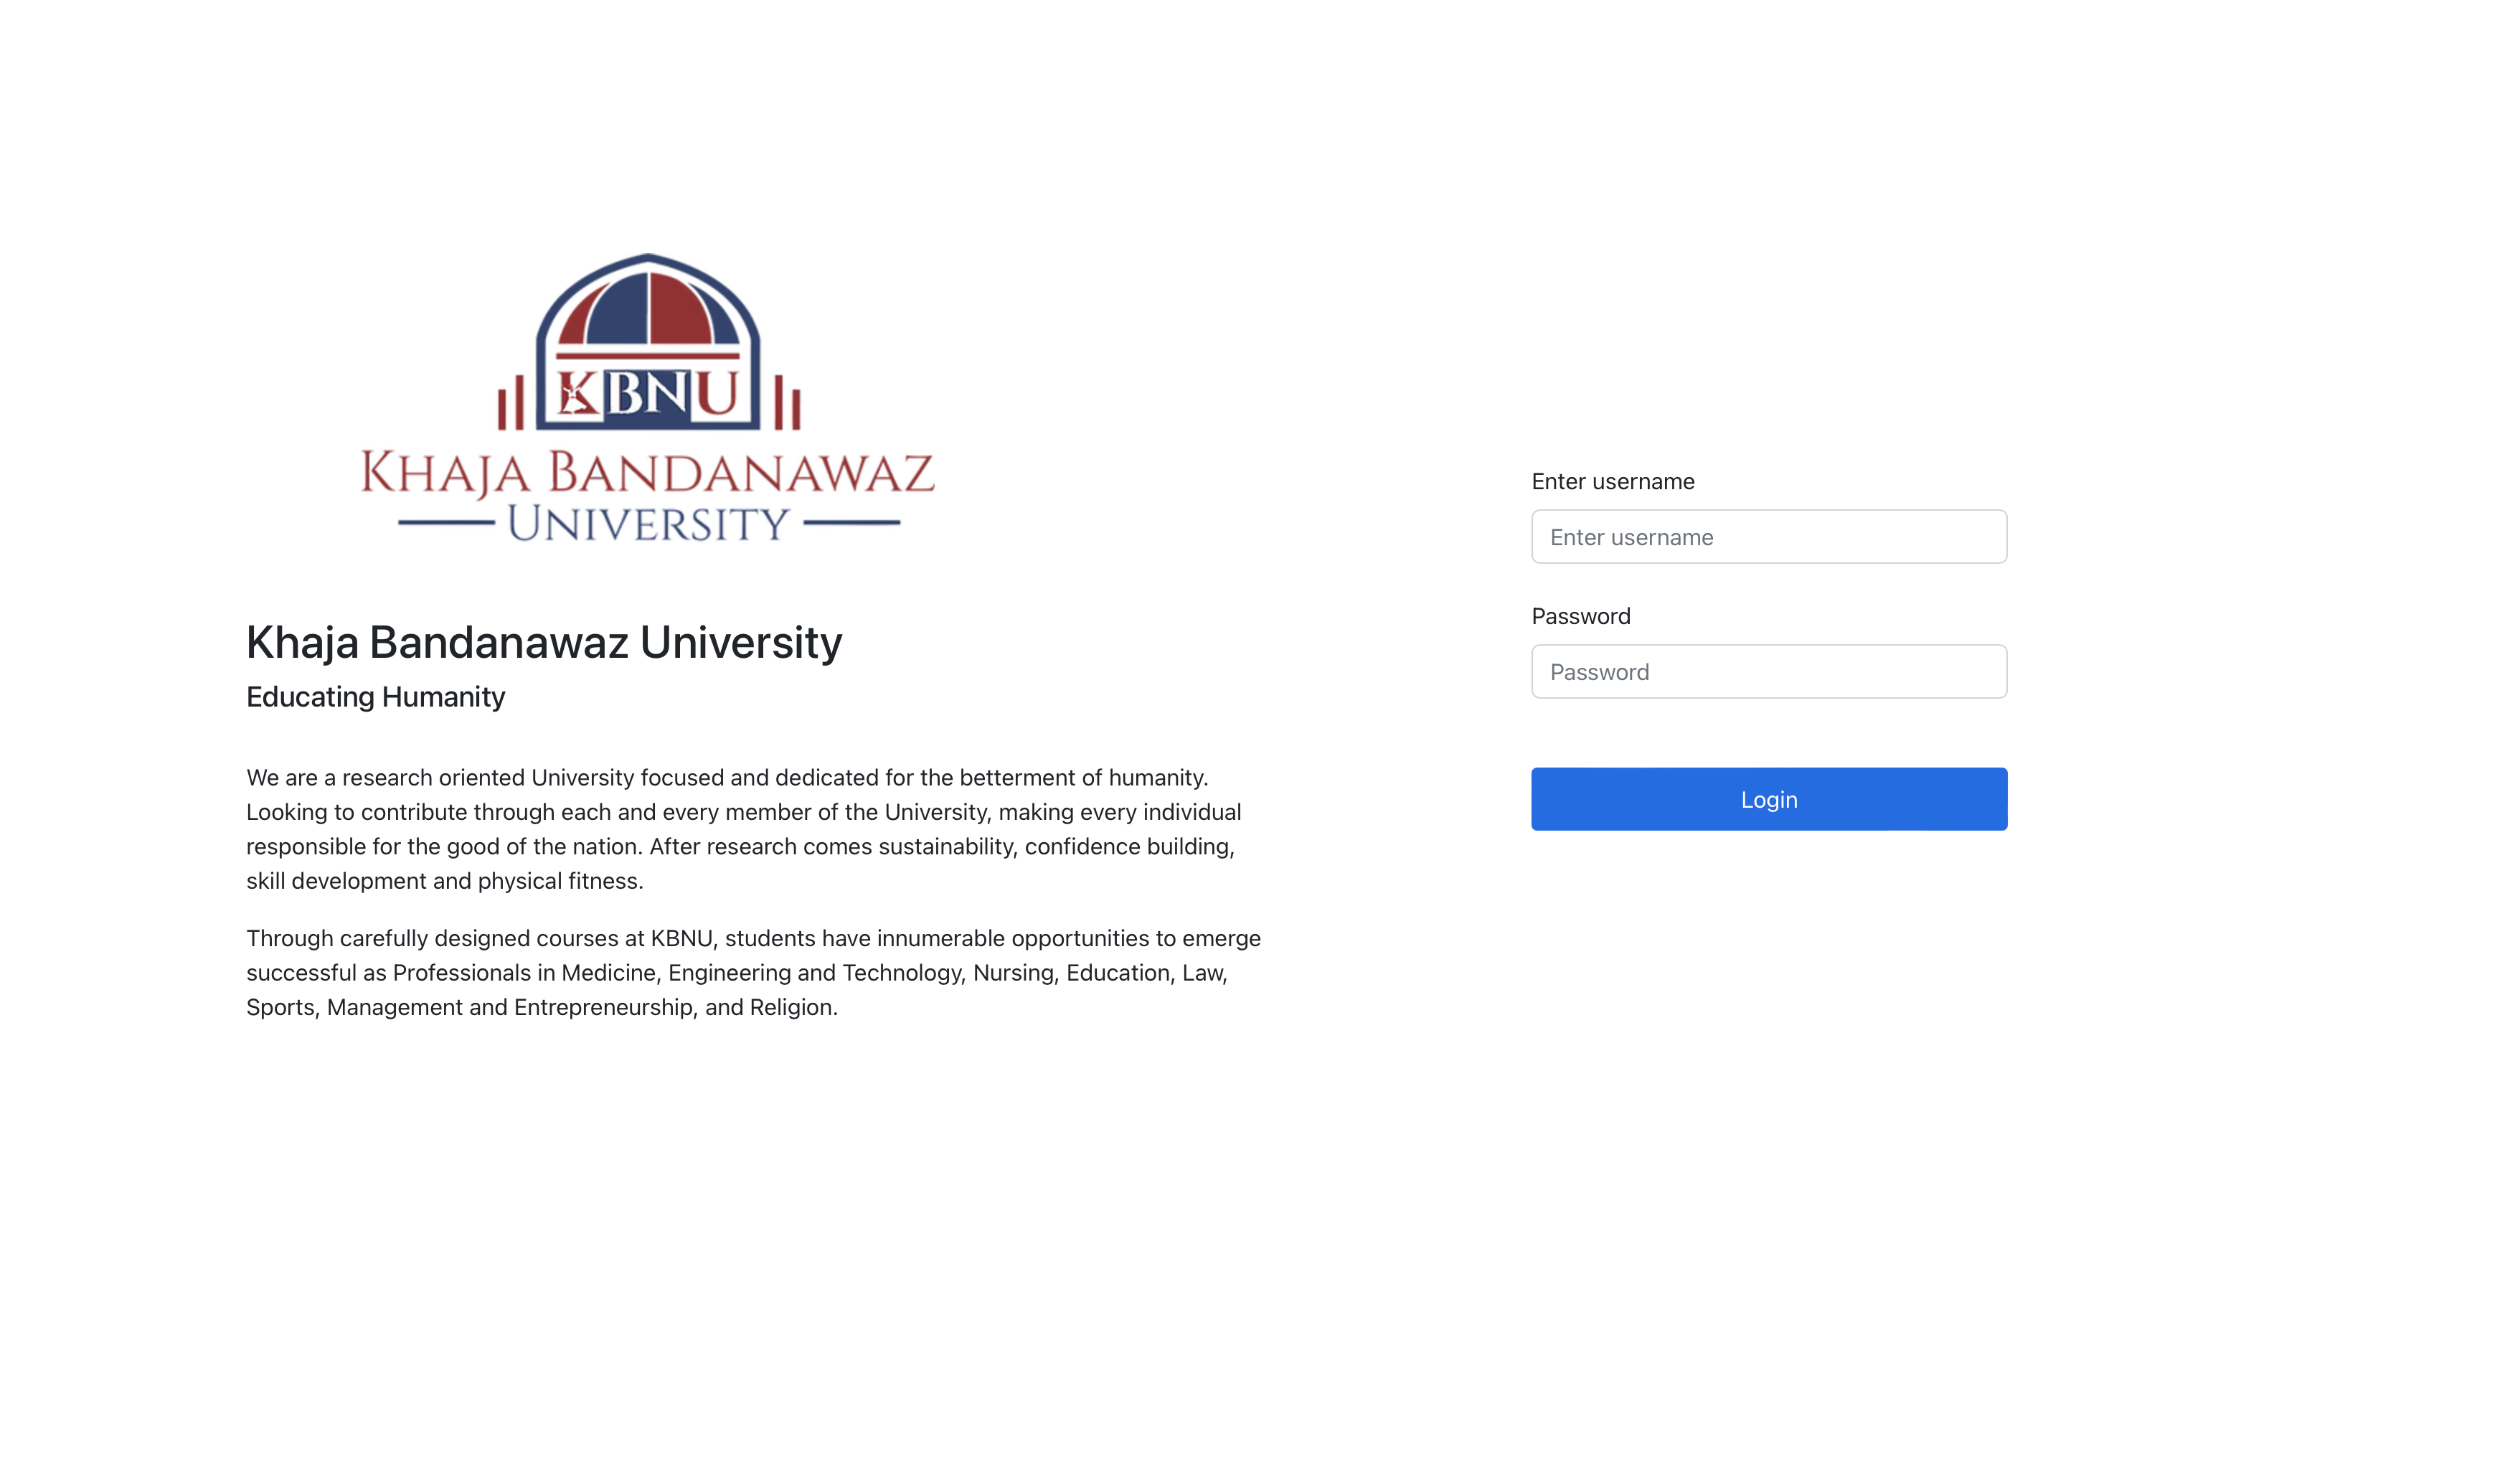
\includegraphics[
        keepaspectratio=true,
        width=15cm
    ]{assets/login.png}
    \captionof{figure}{Home page, Login page}
\end{center}

The above shown figure is the first page that the users will interact with, this
is the login page. We do not provide a sign up functionality, as in a university
there is no way just anyone can turn up to and create an account, it is only
created by the admin.

When a student logs in into the system, he/she is presented with the below shown
page, here on this page the student can see their details, and on the side bar
there is a space for their profile picture, name, university number. There are
buttons on the side bar shown which are used to go to other pages.

\begin{center}
    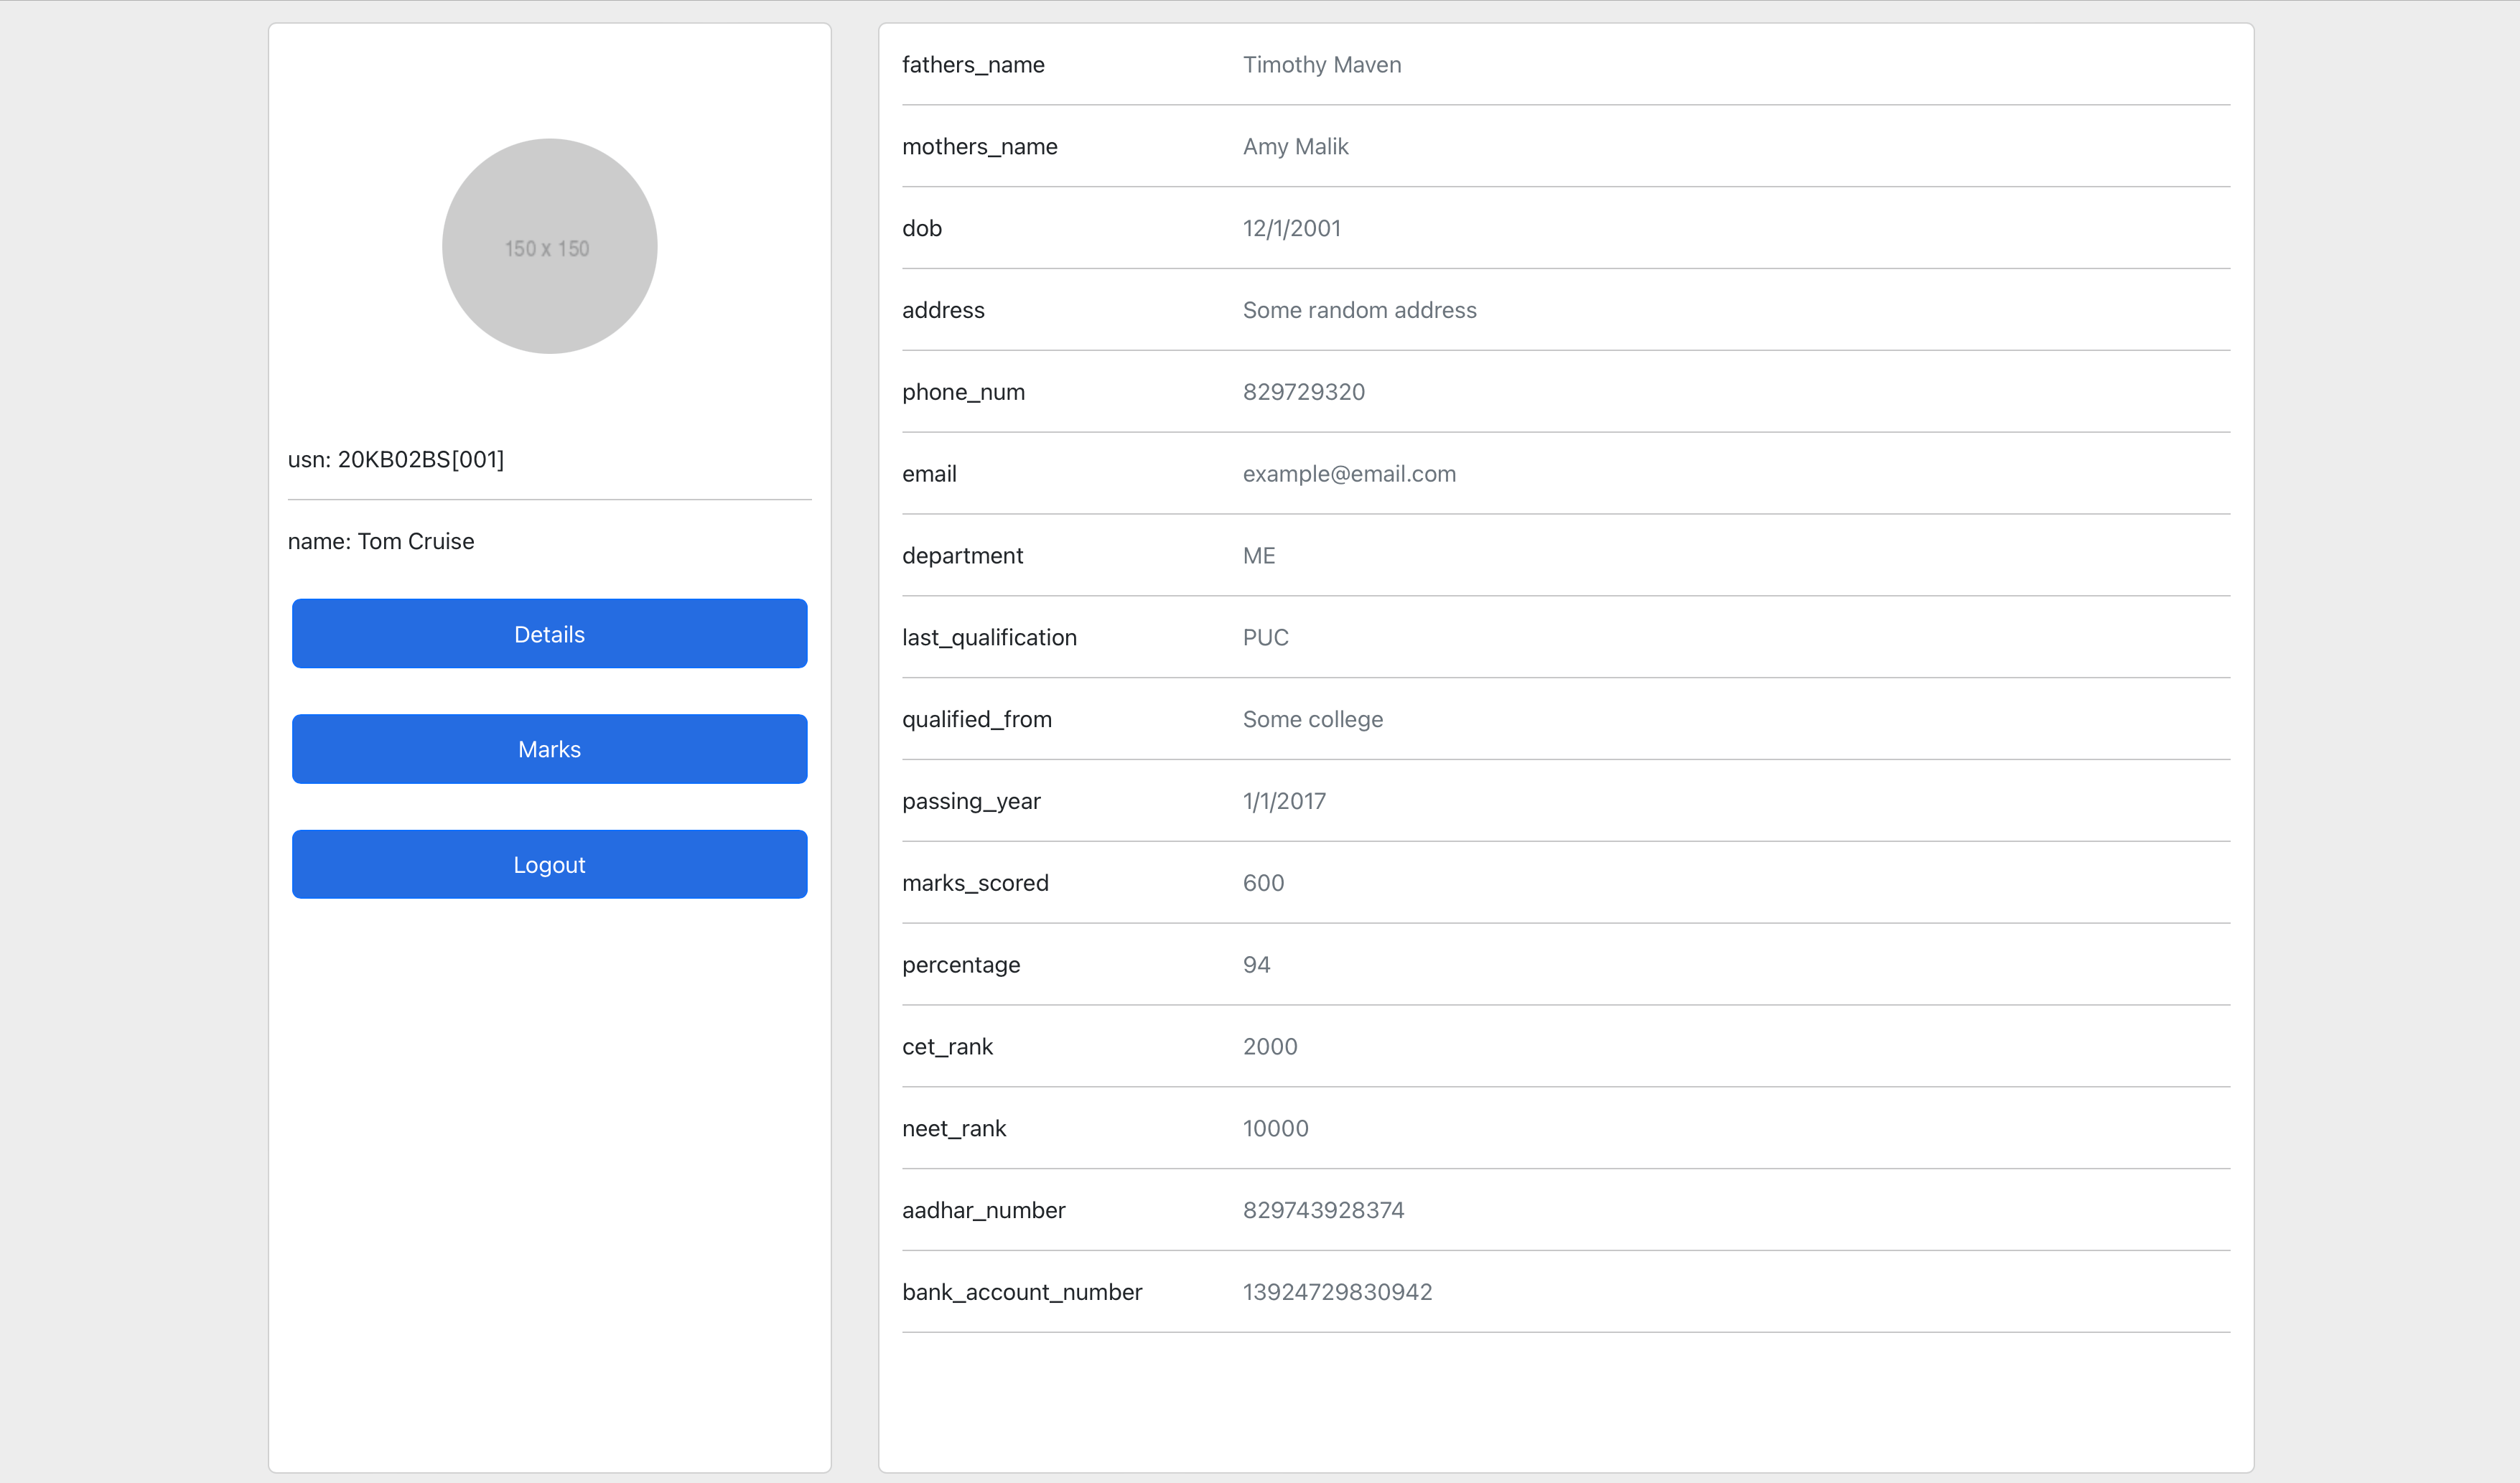
\includegraphics[
        keepaspectratio=true,
        width=15cm
    ]{assets/stud-details.png}
    \captionof{figure}{Students home page}
\end{center}

The details page contains, as the name implies, all of the details that were
previously shown in the table description section, for the student that has just
logged in. The client is required to make additional requests to the API for the
required details, depending upon authorization of requests the data is shown.

\begin{center}
    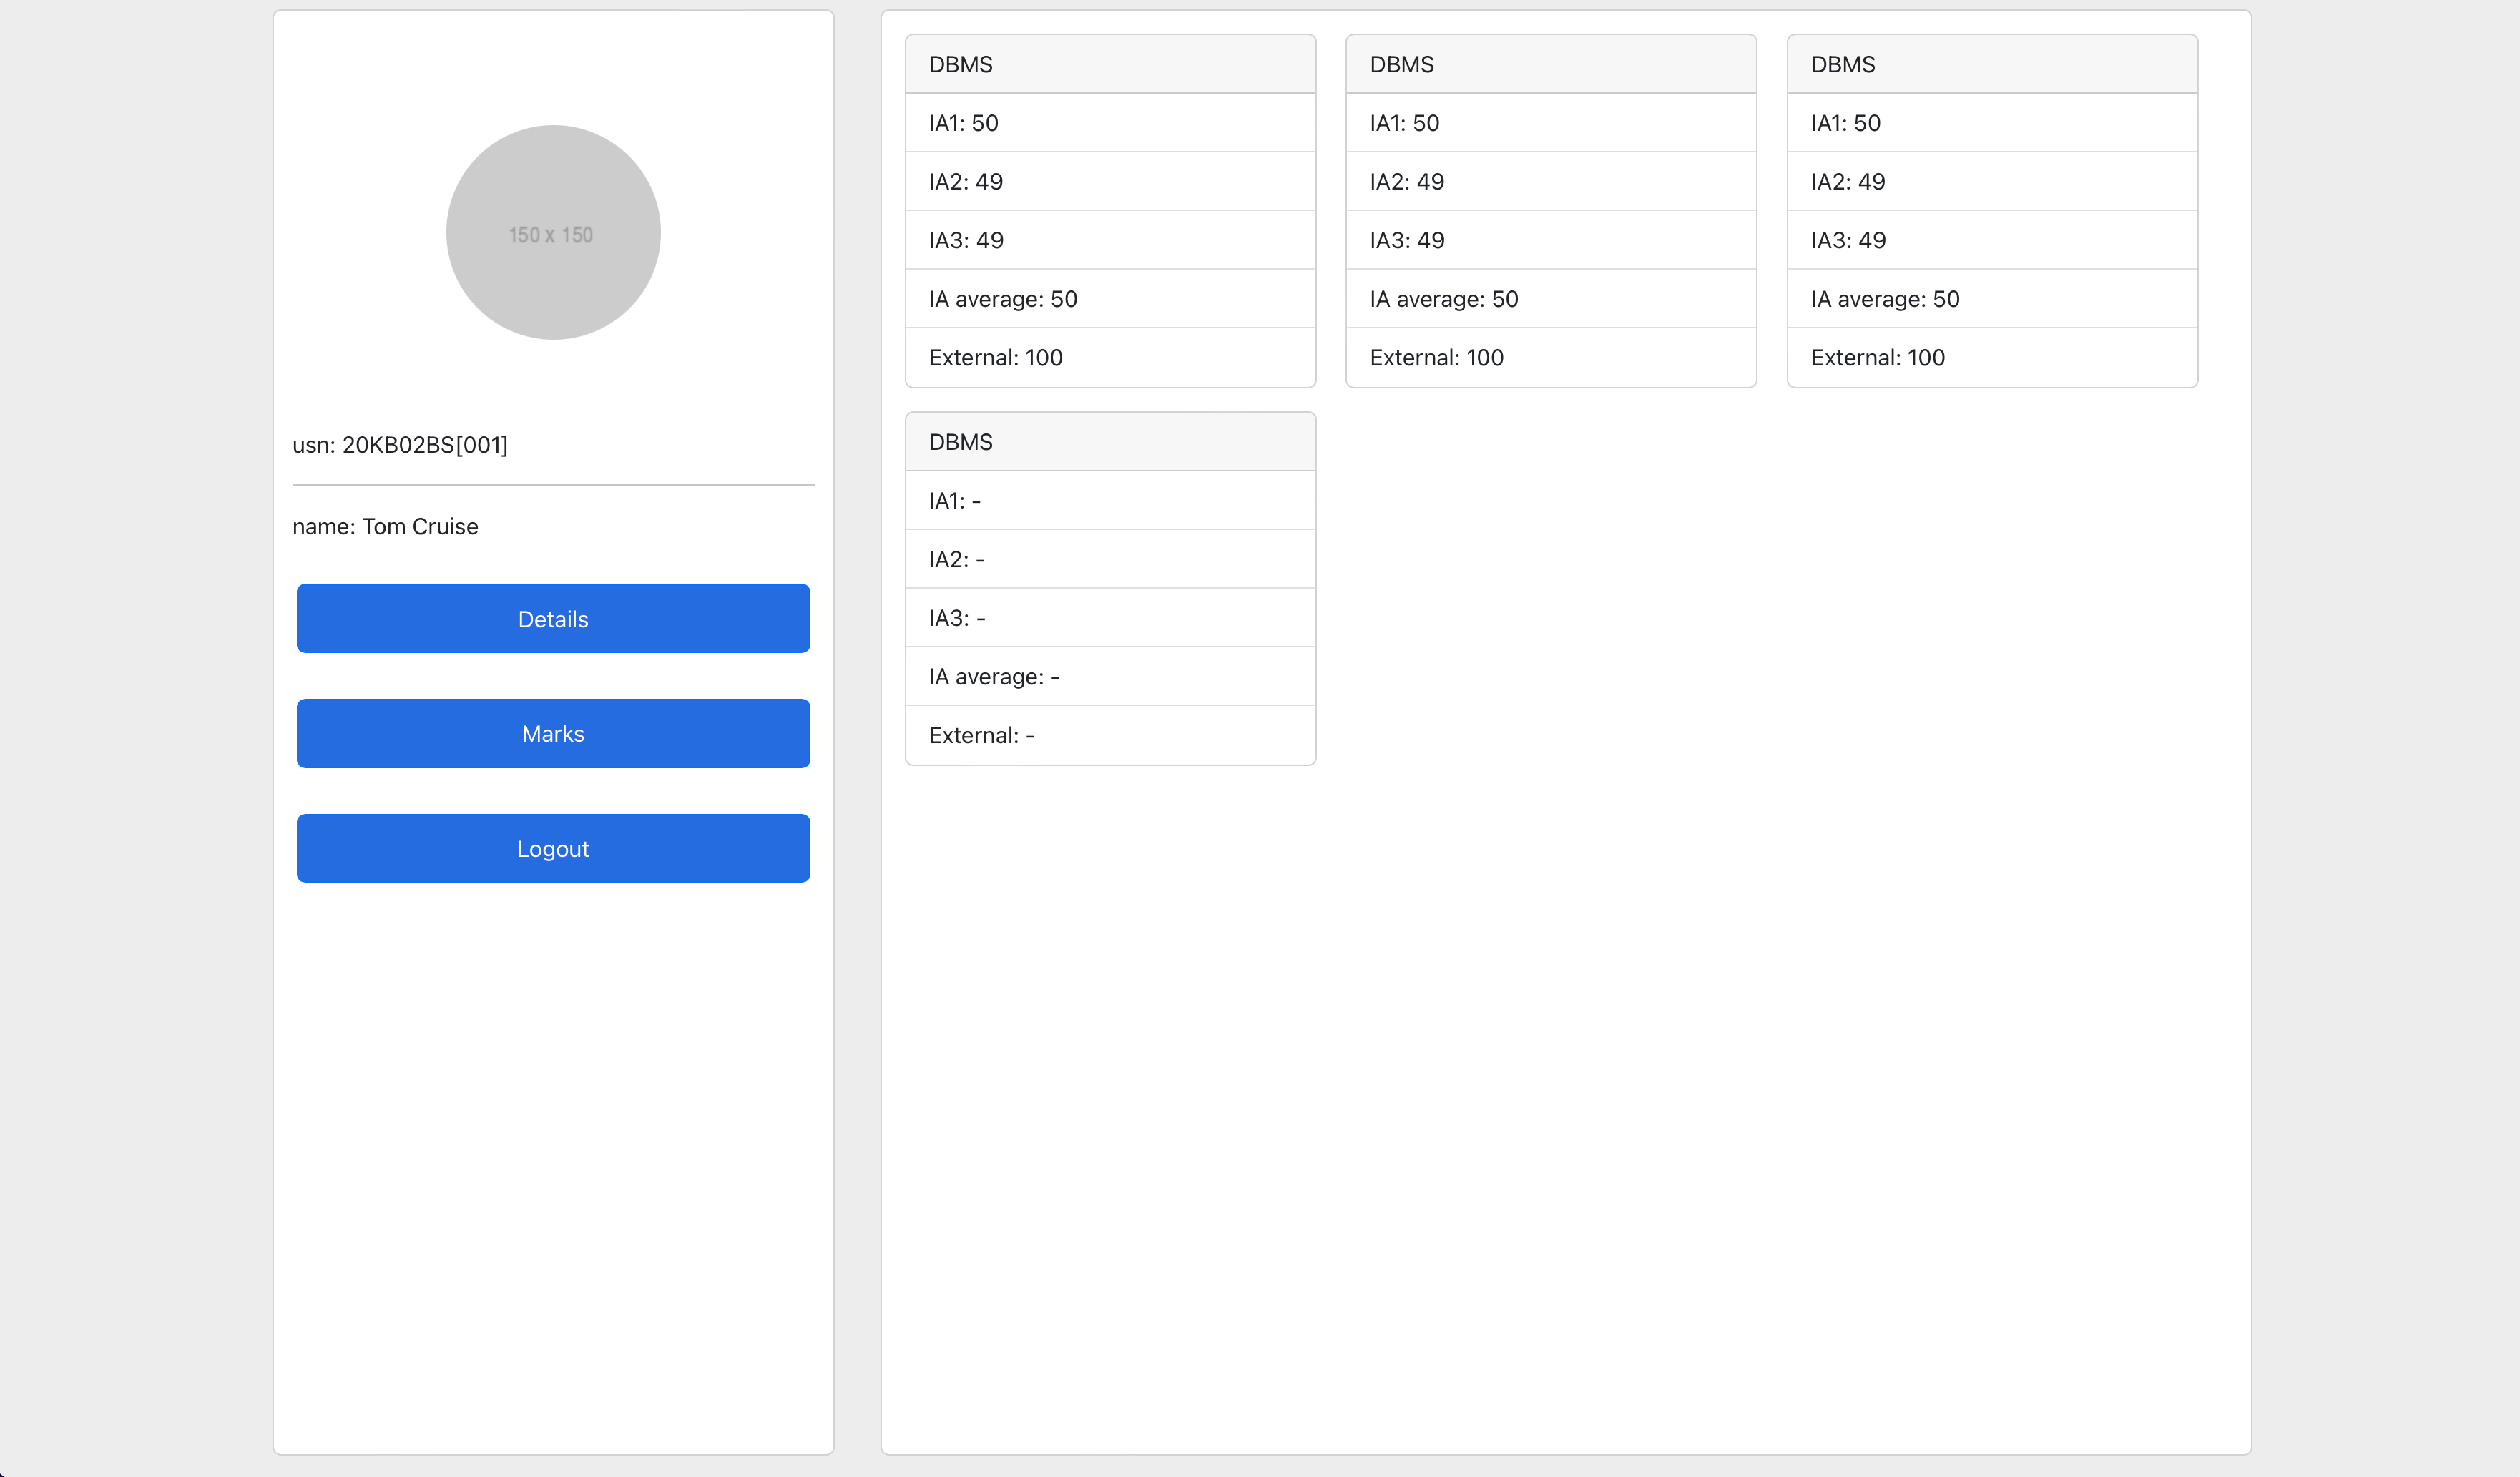
\includegraphics[
        keepaspectratio=true,
        width=15cm
    ]{assets/stud-marks.png}
    \captionof{figure}{Students marks page}
\end{center}

When the student clicks on the "Marks" tab, he/she will be taken to page shown
in figure 3, which shows all of their marks for various subjects assigned to
them. The student can go back to their profile page and also logout.

\begin{center}
    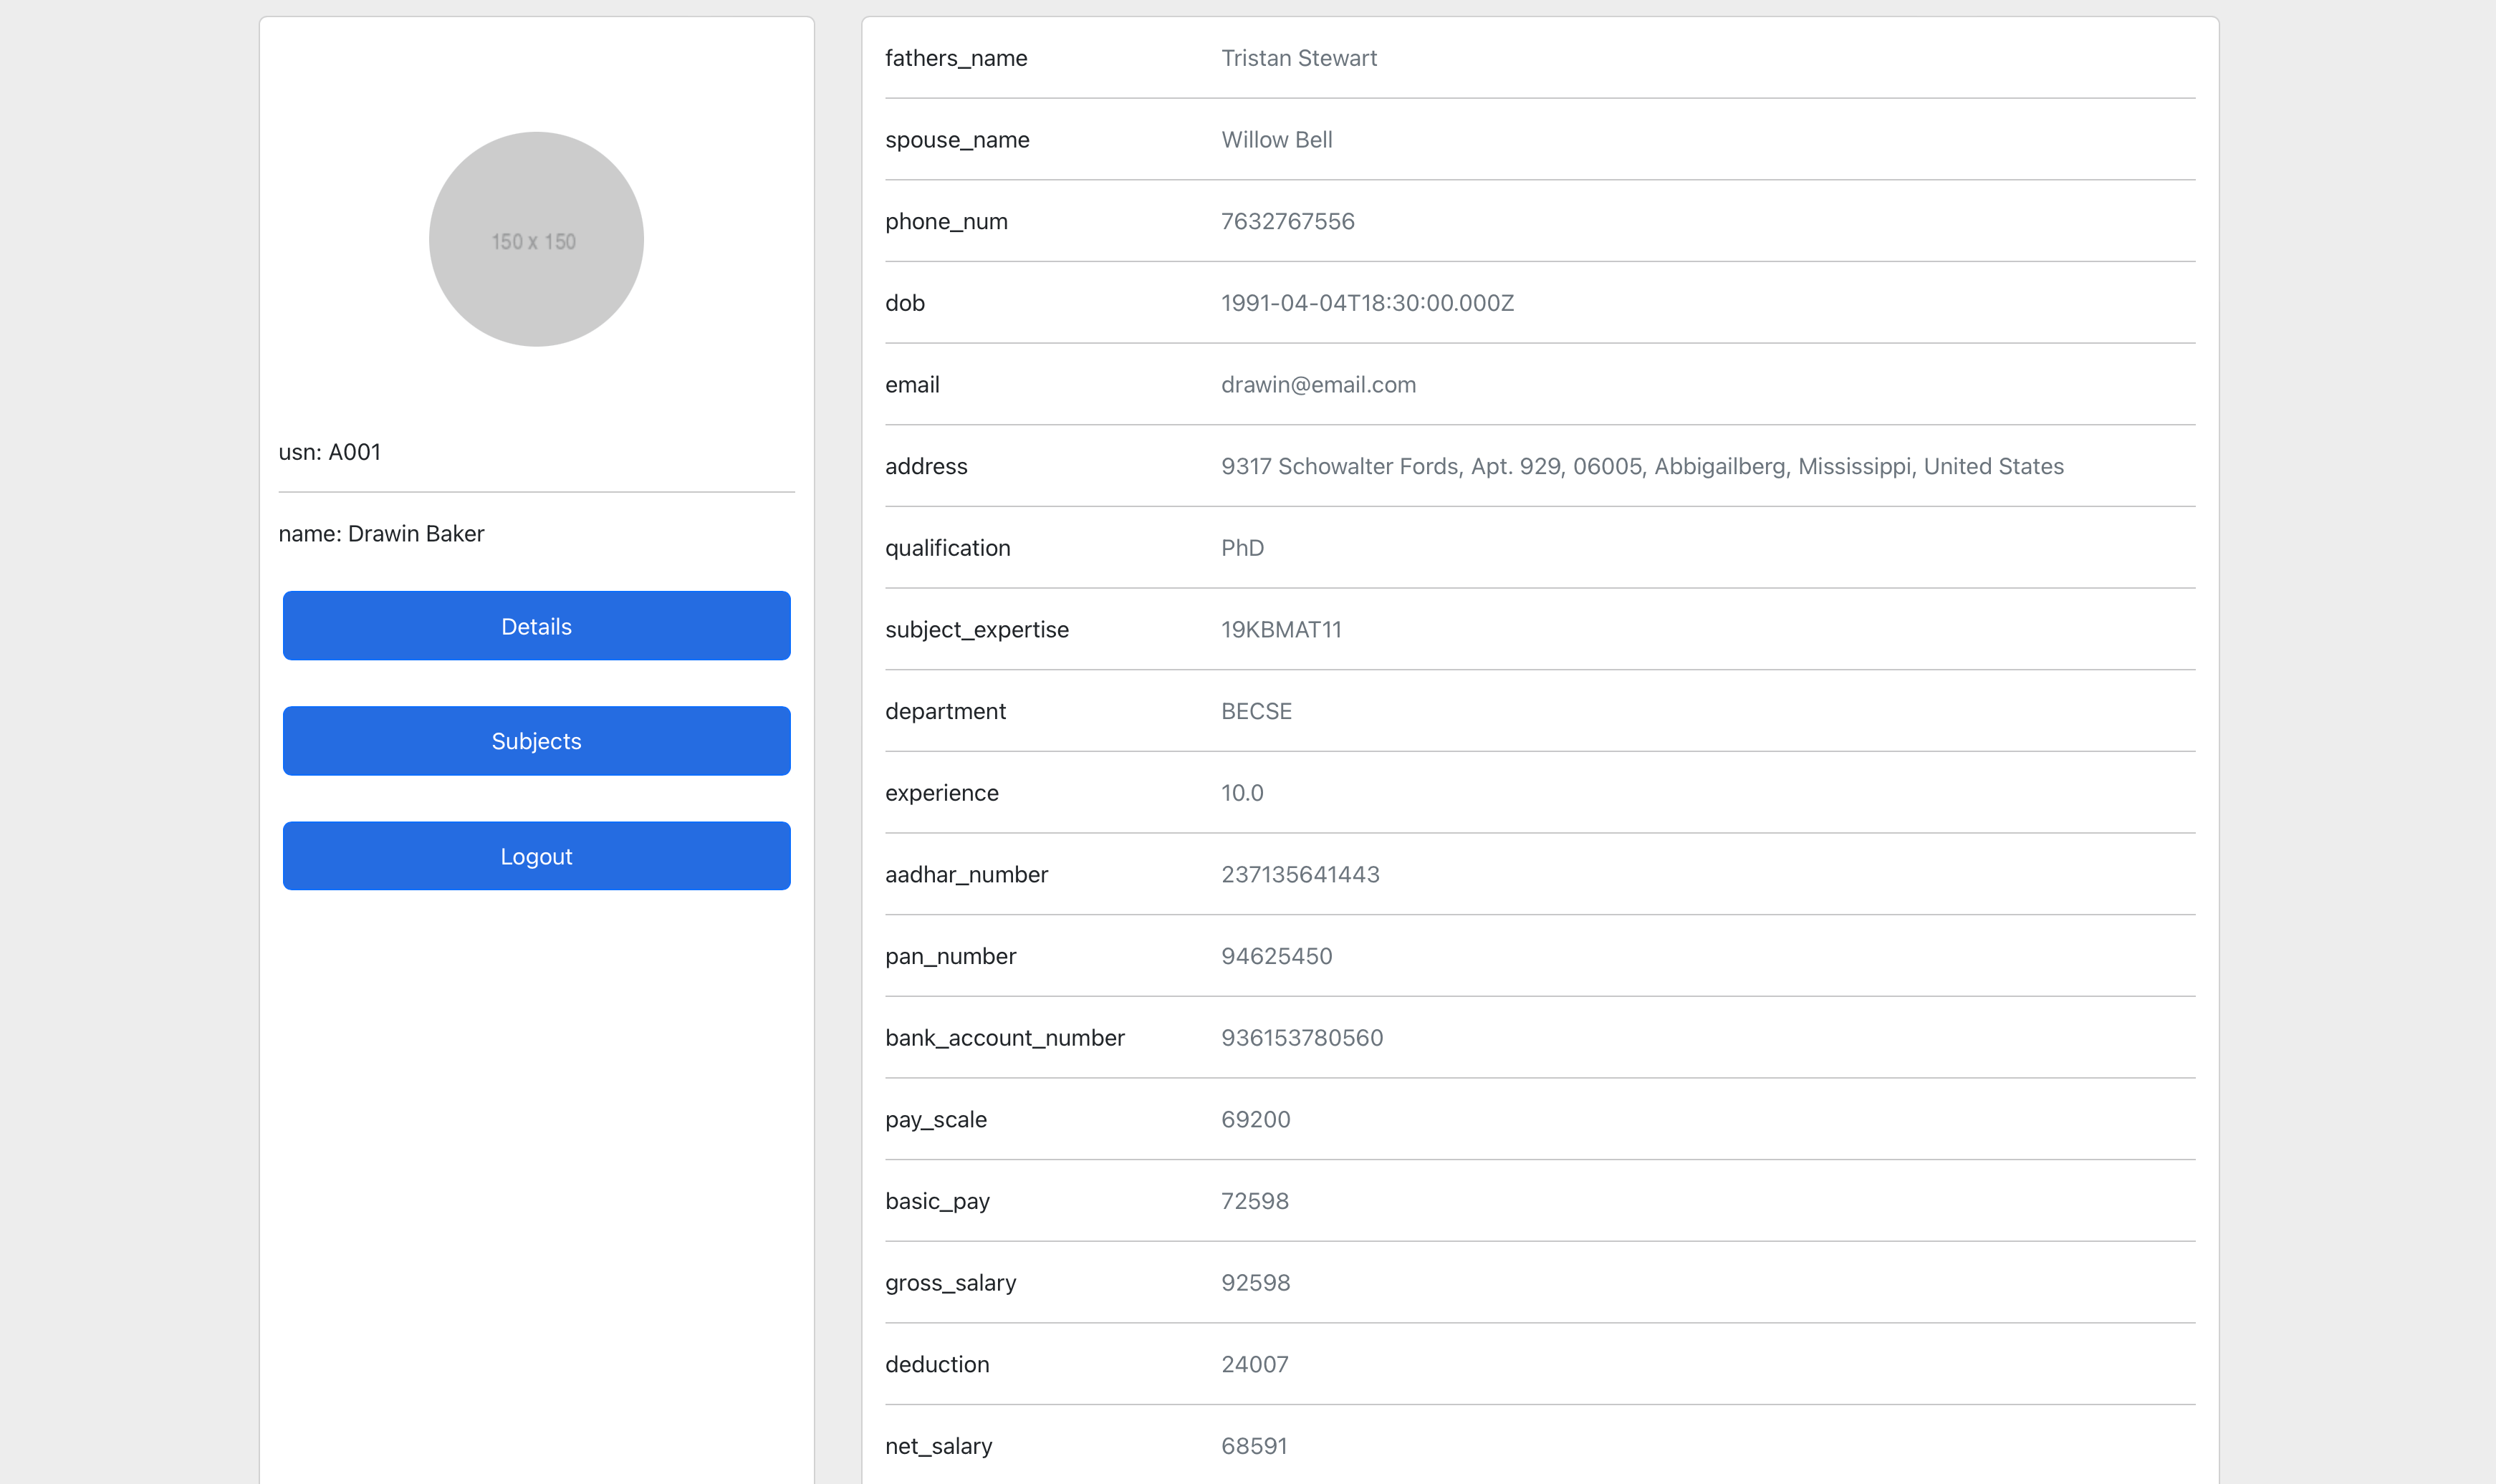
\includegraphics[
        keepaspectratio=true,
        width=14cm
    ]{assets/lect-details.png}
    \captionof{figure}{Lecturers home page}
\end{center}

When a faculty logs in into the system, they are presented with the same details
page as of students, but with details that are for that faculty, the side bar
however is different, in here the faculty is given more options as there is a
lot more work that is done by them.

Following are some of the public API routes that return the information that is
publicly available.

\begin{center}
    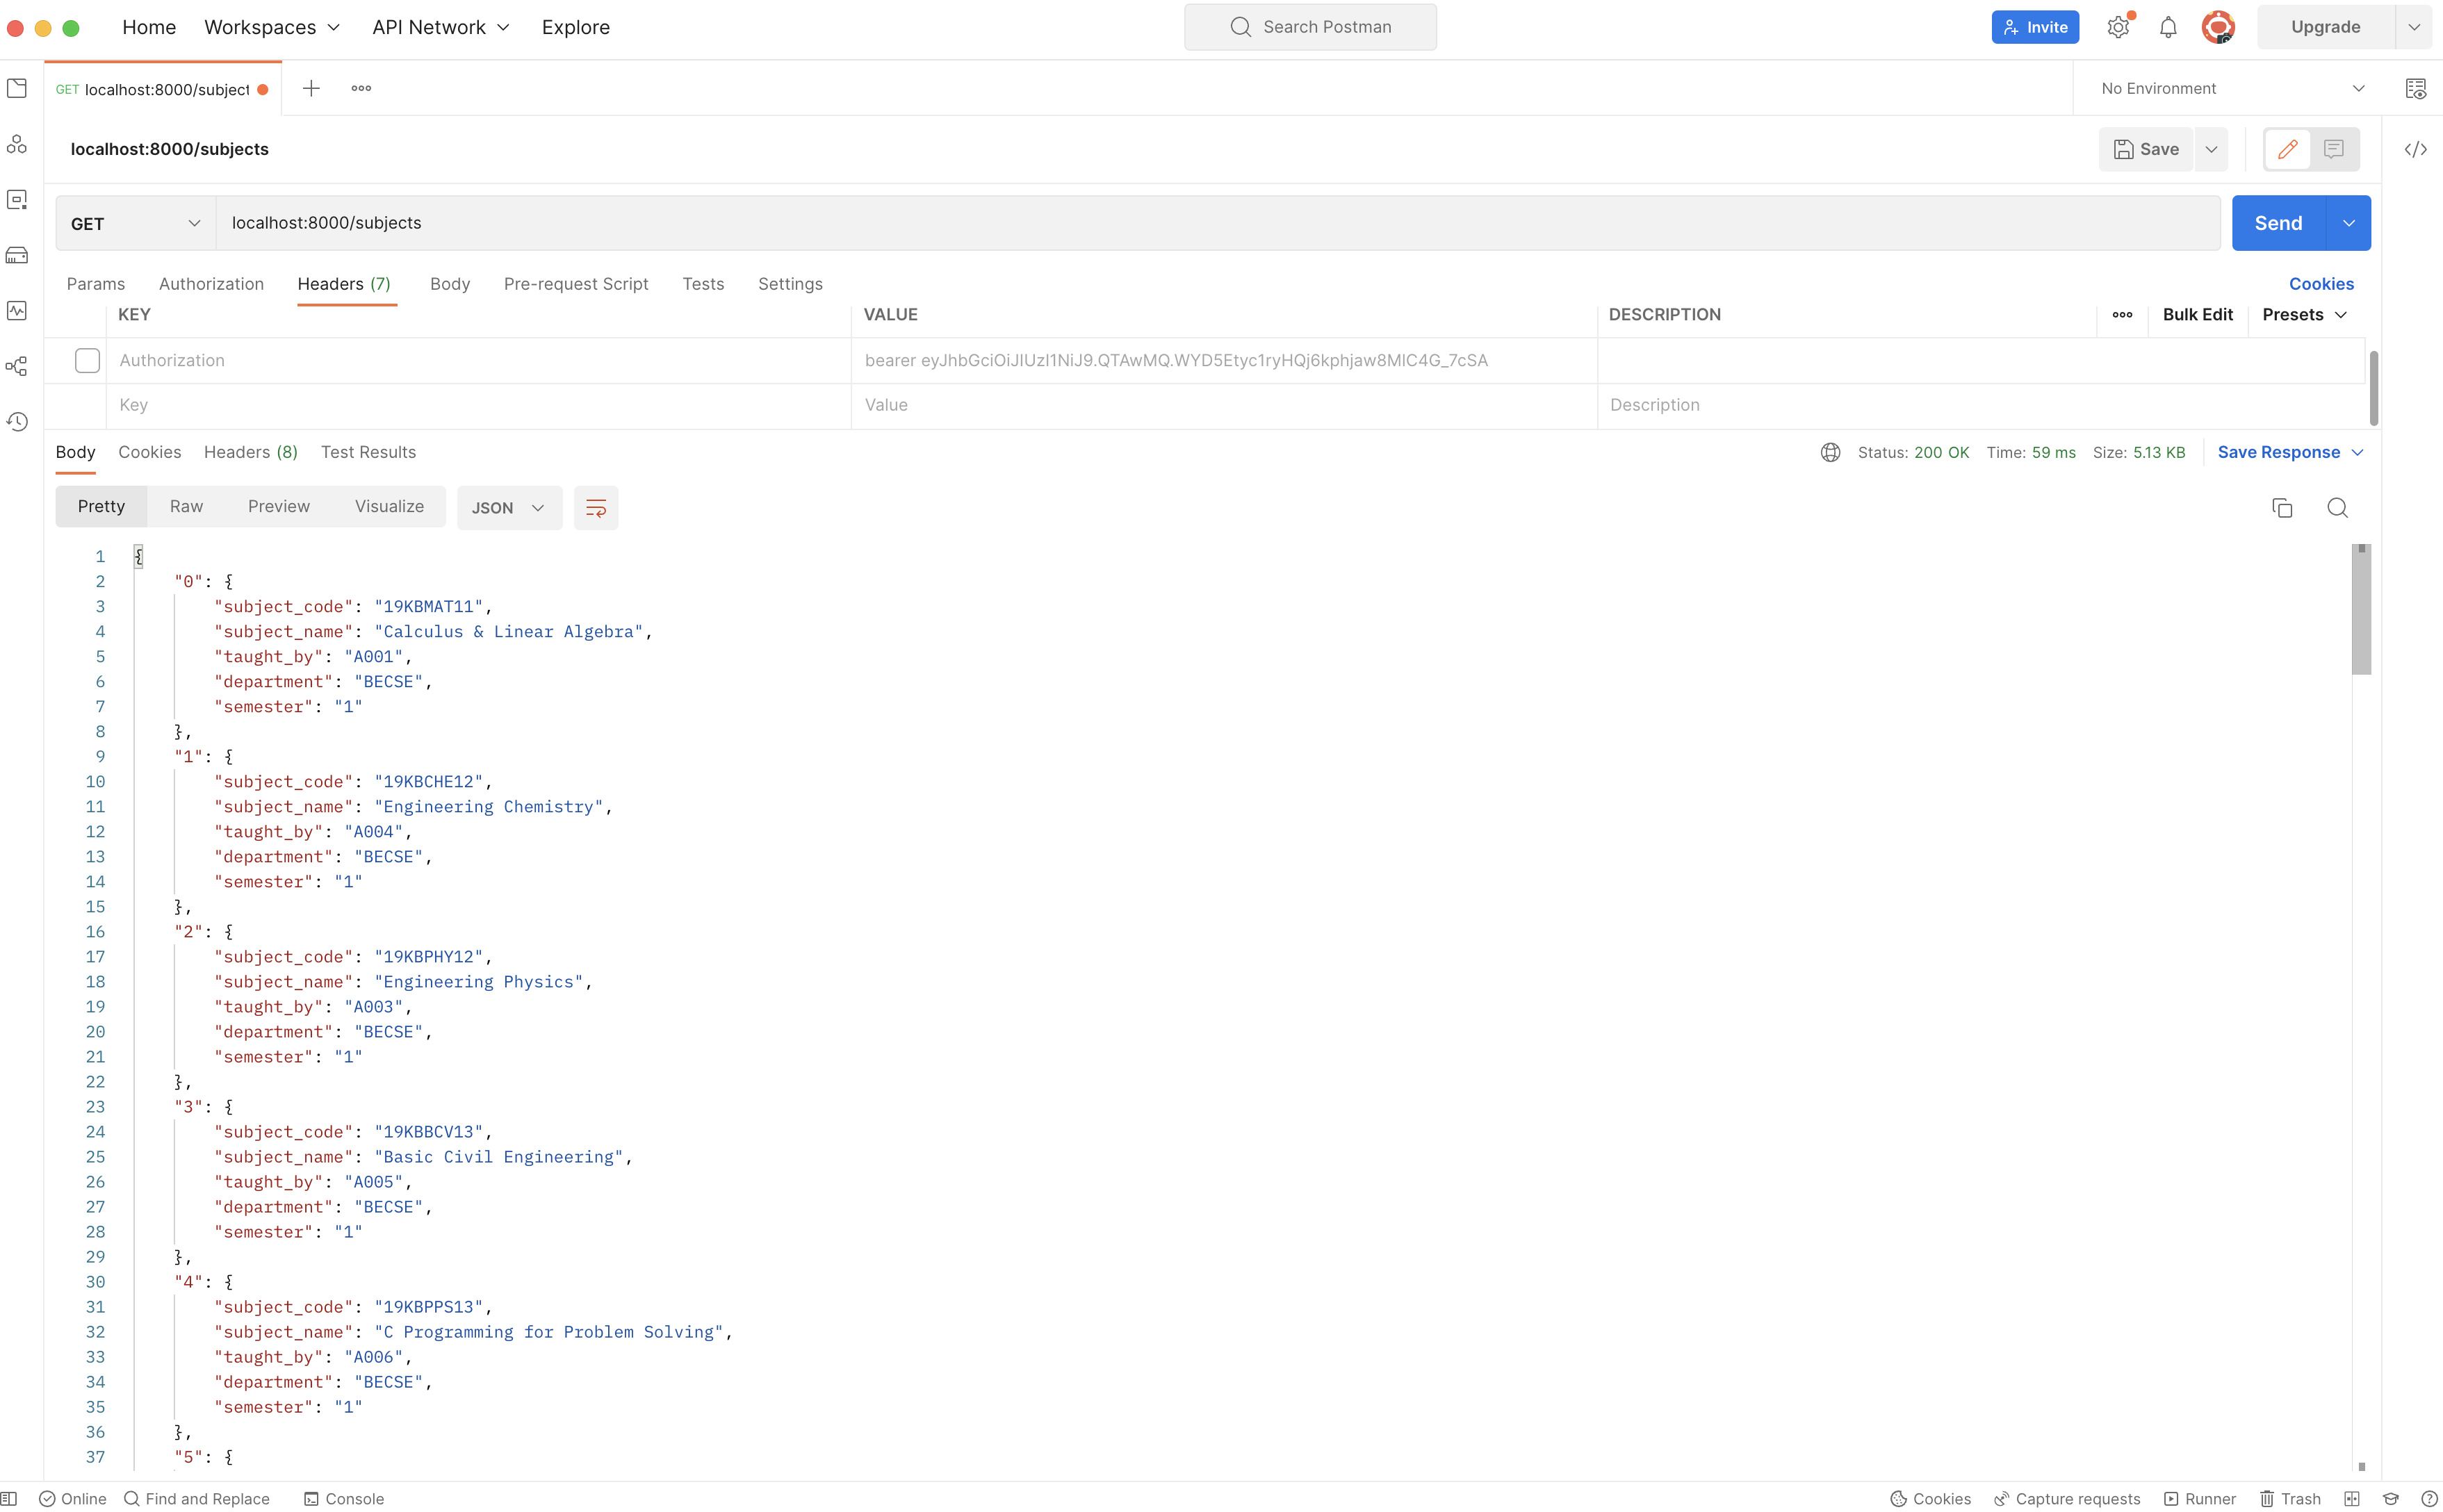
\includegraphics[
        keepaspectratio=true,
        width=14cm
    ]{assets/subjects-api.png}
    \captionof{figure}{API route returning all subjects}
\end{center}

The subjects API route returns all of the subjects that are taught in the
university, across various departments

\begin{center}
    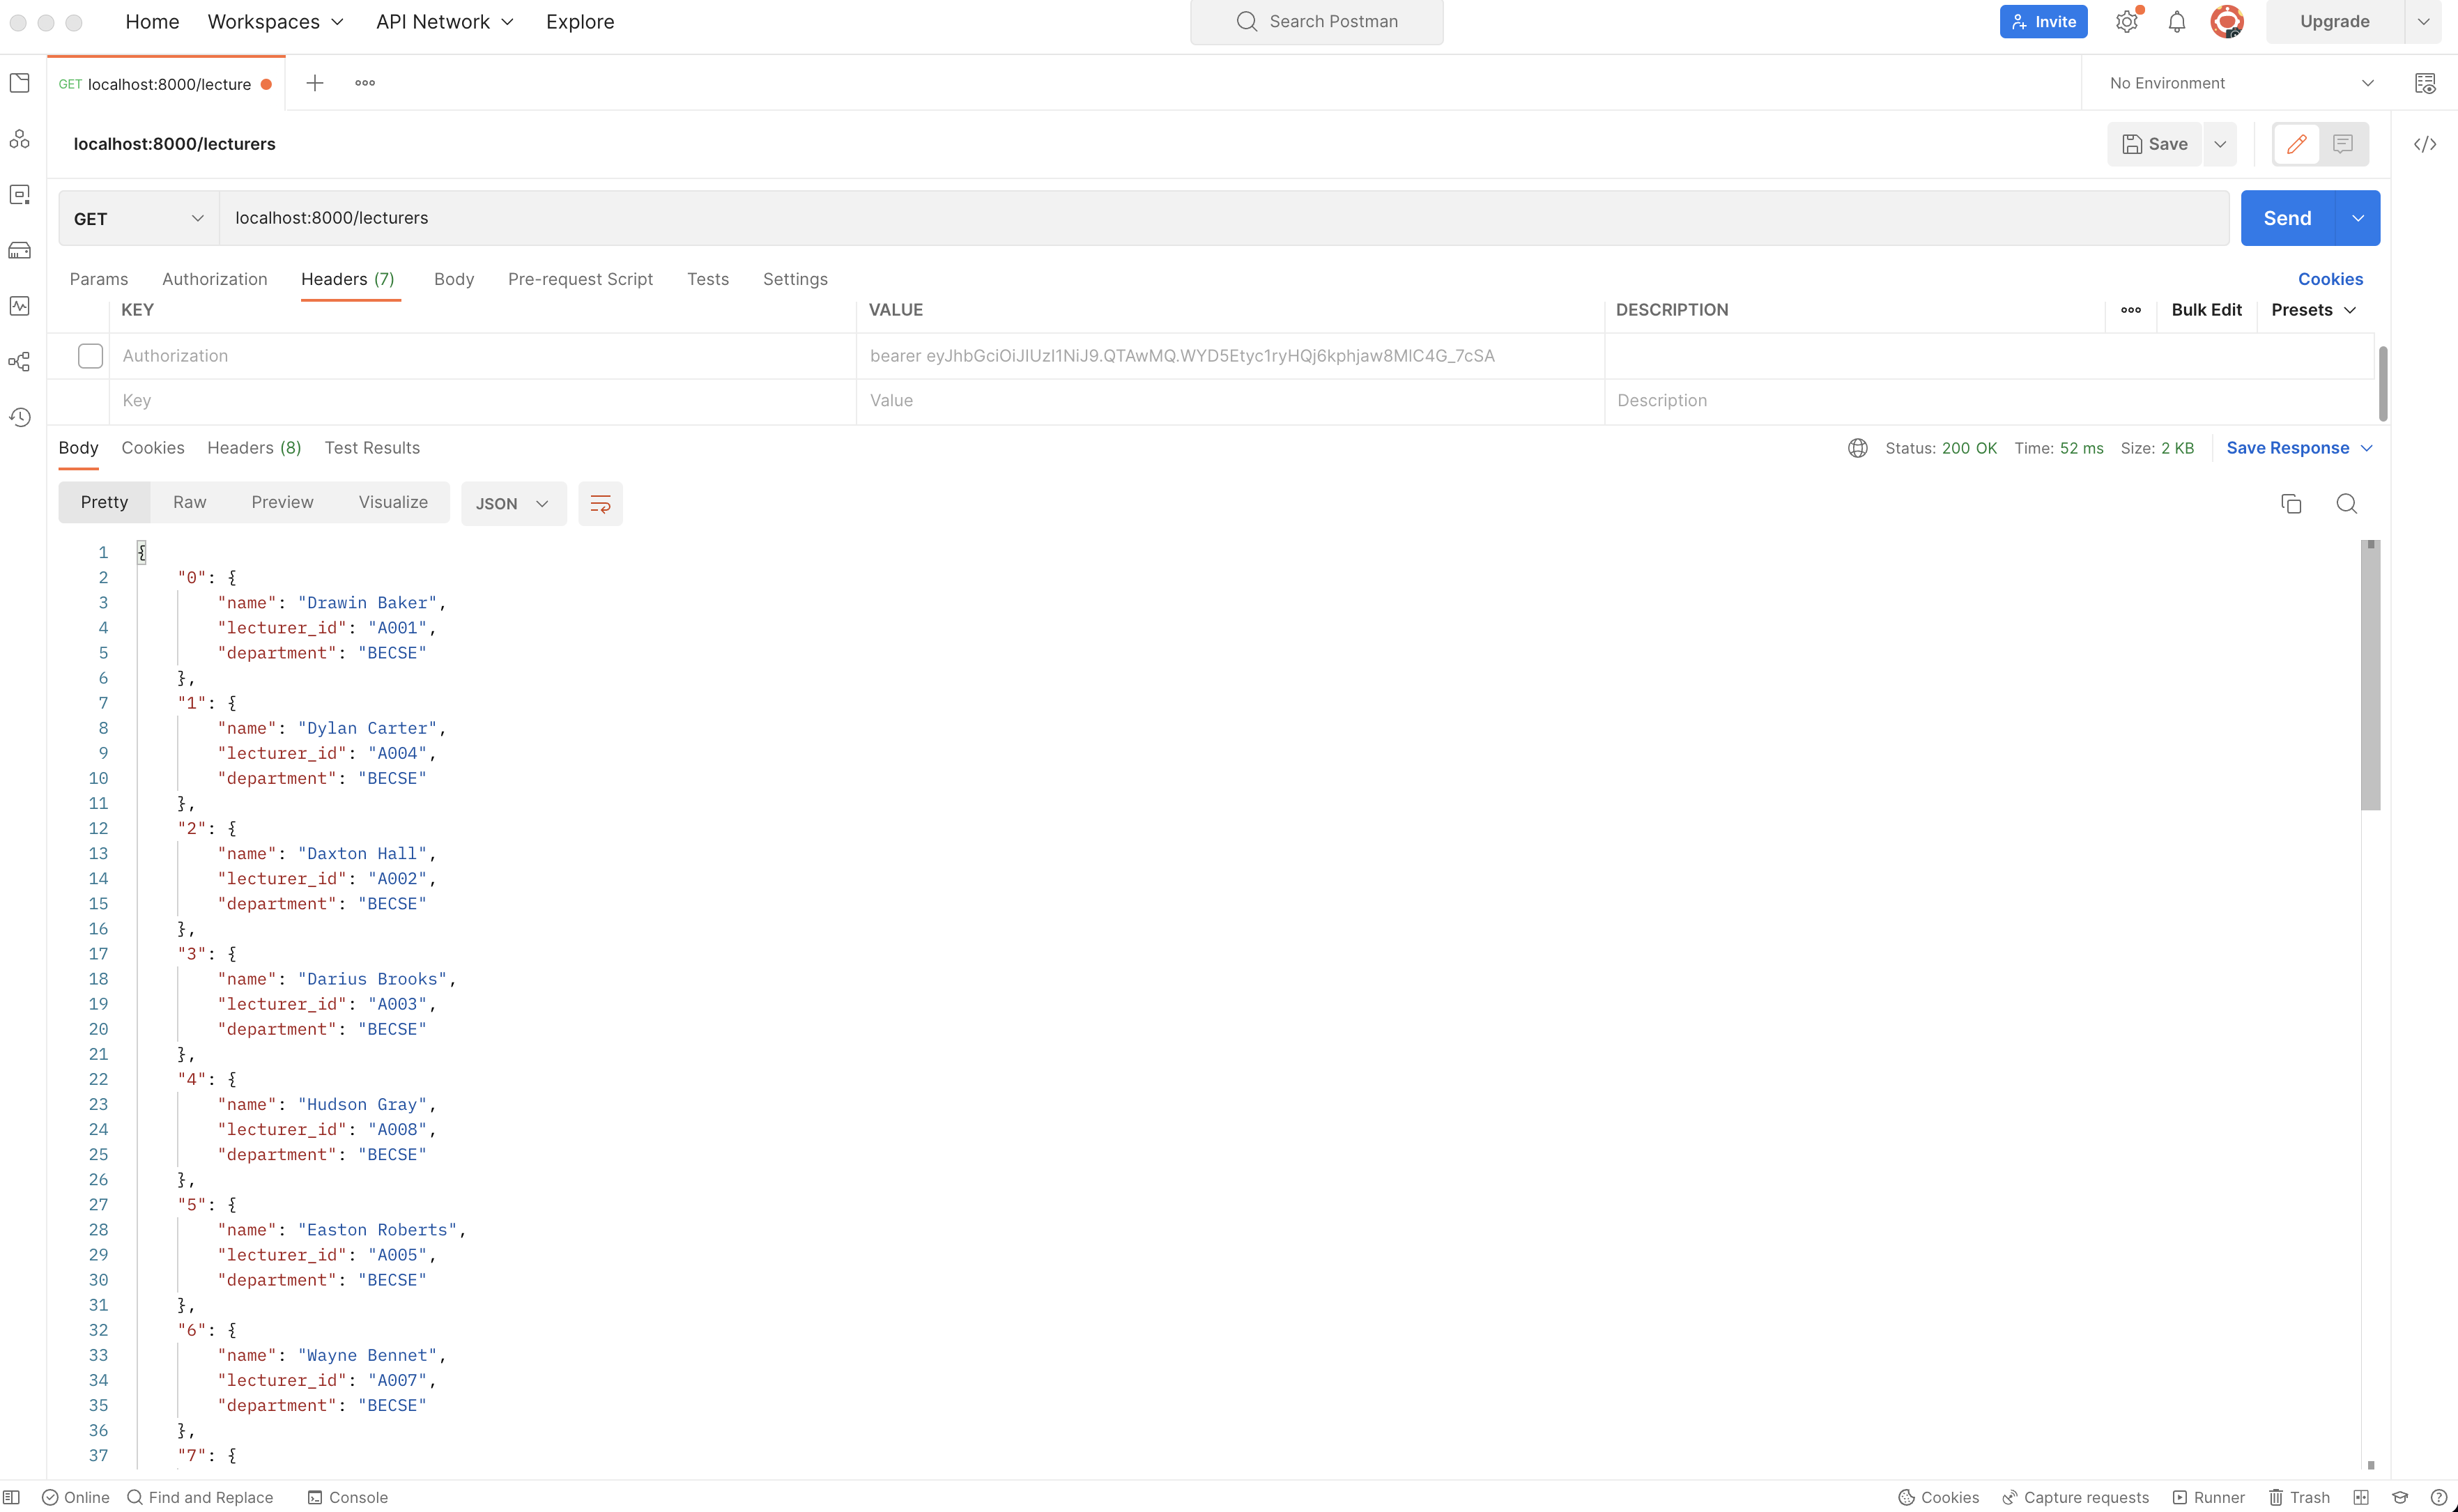
\includegraphics[
        keepaspectratio=true,
        width=14cm
    ]{assets/lecturers-api.png}
    \captionof{figure}{API route returning all lecturers}
\end{center}

The lecturers API route return the information about all lecturers that teach
in a university, since this route is public it does not return any sensitive
information.

\begin{center}
    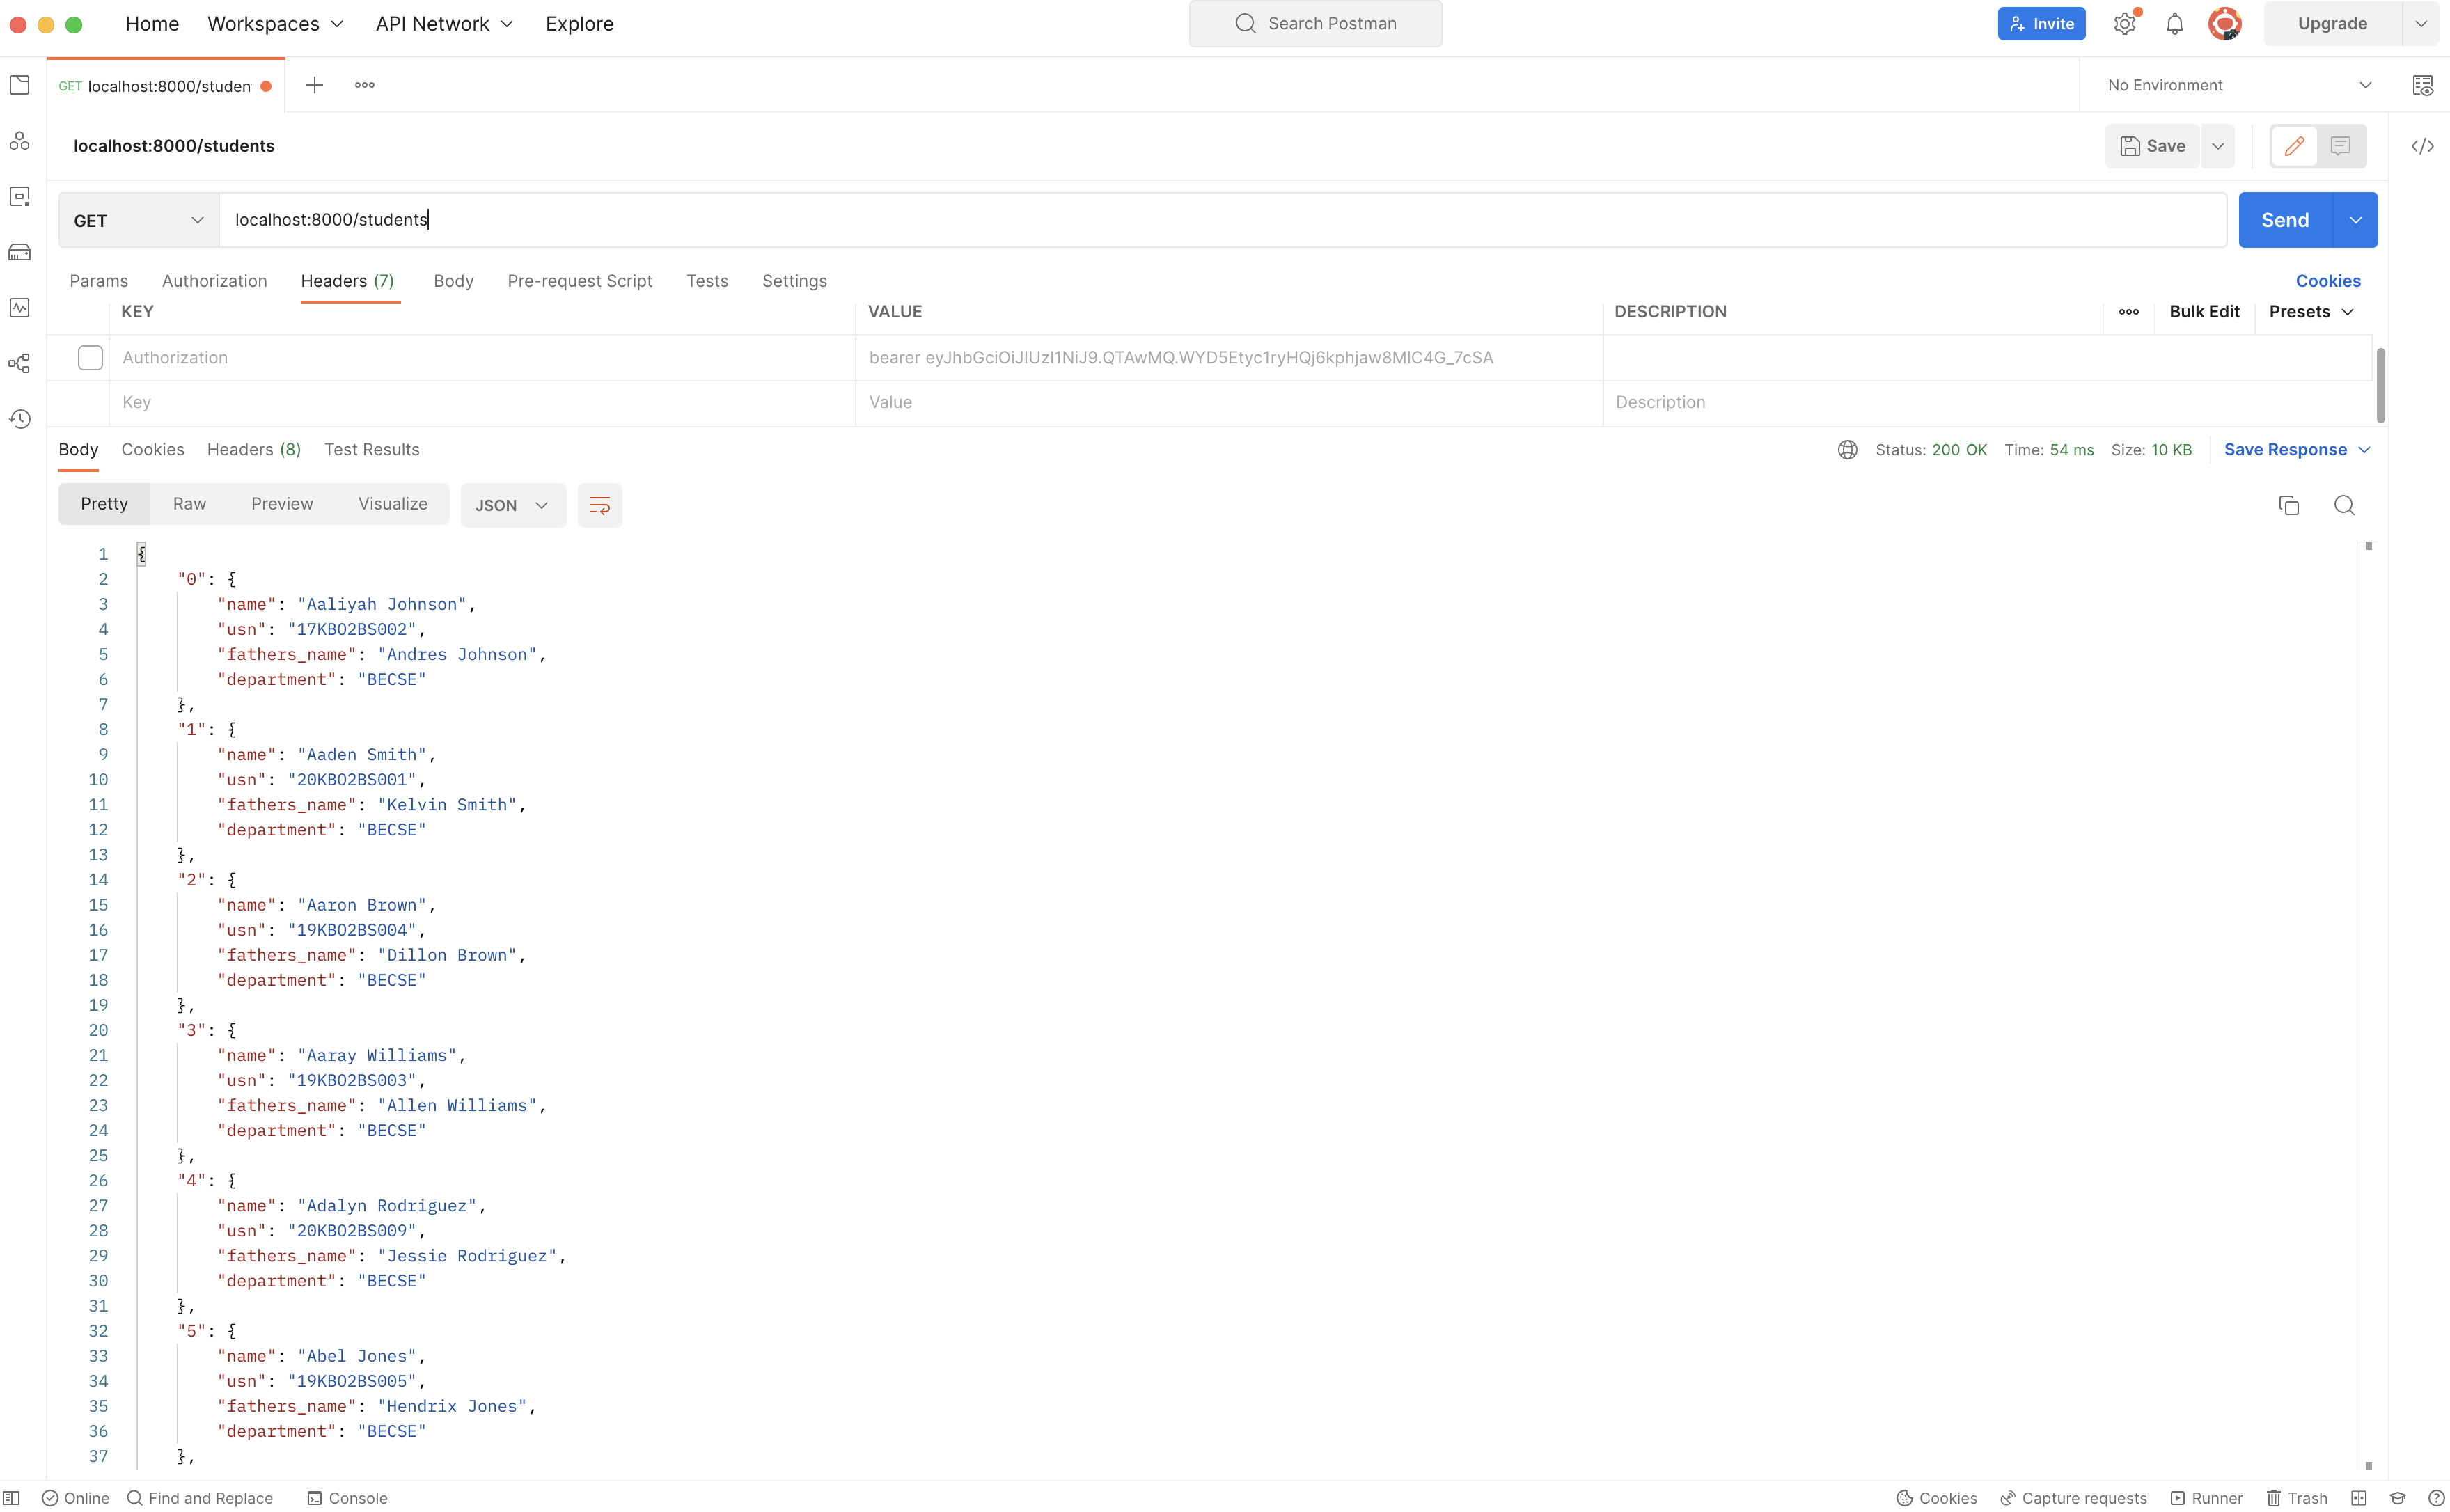
\includegraphics[
        keepaspectratio=true,
        width=14cm
    ]{assets/student-api.png}
    \captionof{figure}{API route returning all students}
\end{center}

The students API route return the information about all students that study
in a university, since this route is public it does not return any sensitive
information.
